\documentclass[11pt,italian]{article}
\usepackage[T1]{fontenc}
\usepackage[utf8]{inputenc} %utf8 % lettere accentate da tastiera
\usepackage[italian]{babel} % lingua del documento
\usepackage{blindtext}
\usepackage{enumitem}
\usepackage{graphicx}
\usepackage{float}
\usepackage{xcolor}   % for \textcolor
\usepackage[font=small,labelfont=bf,skip=3pt]{caption}
\setlength{\belowcaptionskip}{-10pt}
\usepackage{listings}
\lstset{
    basicstyle=\small\ttfamily,
    columns=fullflexible,
    frame=single,
    breaklines=true,
    postbreak=\mbox{\textcolor{red}{$\hookrightarrow$}\space},
    tabsize=4, % tab space width
    showstringspaces=false, % don't mark spaces in strings
    numbers=left, % display line numbers on the left
    commentstyle=\color[HTML]{a0a1a7}, % comment color
    keywordstyle=\color[HTML]{40a3f5}, % keyword color
    stringstyle=\color{red}, % string color,
    emphstyle={\color[HTML]{40a3f5}}
}

\usepackage{hyperref}
\usepackage{cleveref}
\hypersetup{
    colorlinks = true,
    linkbordercolor = {white},
    urlcolor = blue
}
\usepackage{graphicx}
\graphicspath{ {./images/} }

% Italian syntax spacing
\frenchspacing

% Line height
\renewcommand{\baselinestretch}{1.15}

\title{
    Metodi del Calcolo Scientifico \\
    \normalsize Risoluzione di sistemi lineari tramite il metodo di Cholesky \\
}

\date{\small A.A. 2019/2020}

\author{
    \normalsize
    \textsc{Edoardo Silva} 816560 \\
    \normalsize
    \textsc{Bryan Zhigui} 816335 \\
    \normalsize
    \textsc{Davide Marchetti} 815990
}

\begin{document}

\maketitle

\section*{Abstract}
Questo progetto si prefigge lo scopo di studiare l'implementazione del metodo di Choleski per la risoluzione sistemi lineari per matrici simmetriche defite positive sparse in un ambiente di programmazione open source e di compararli con l'implementazione closed-source di MATLAB.

Il confronto avverrà in termini di tempo, accuratezza, impiego della memoria e anche facilità d'uso sia in ambiente Linux che Windows, eseguendo il codice su diverse matrici derivate da problemi reali e raccolte nella \textbf{SuiteSparse Matrix Collection}\footnote{\url{https://sparse.tamu.edu/}}.

\newpage
\section{Analisi dell'implementazione}

\subsection{MATLAB}
Per la decomposizione di cholesky, MATLAB mette a disposizione il modulo \textbf{cholesky.matlab} contenente tutto il necessario. In particolare è stata utilizzata la funzione \textbf{chol}

\subsubsection*{Utilizzo}
\lstinline{R = chol(A, [triangle])}: Fattorizza la matrice $A$ simmetrica definita positiva in una matrice triangolare superiore $R$ tale che $A=R^{-1}R$.
Il parametro \lstinline{triangle} permette di scegliere se attuare la decomposizione in una matrice triangolare superiore (opzione di default) o traiangolare inferiore. In quest'ultimo caso, la matrice $R$ risultante dall'equazione soddisferà l'uguaglianza $A = RR^{-1}$.

\subsubsection*{Manutenzione}
La libreria è stata rilasciata per la prima volta nell'aggiornamento R2013a MATLAB. Attualmente, è ancora supportata e non presenta lacune o problemi che sono stati riscontrati durante il suo l'utilizzo.

\subsubsection{Documentazione}
La documentazione ufficiale di MATLAB è ben strutturata e di facile consultazione. Vengono anche proposti molti esempi di utilizzo delle diverse funzioni in varie casistiche.

\subsubsection{Problemi riscontrati}
La criticità principale riguarda il supporto del modulo \lstinline{memory} esclusivamente per sistemi operativi Windows. Difatti, è stato necessario utilizzare due metodi di profiling della memoria diversi a seconda del sistema operativo.

\subsubsection*{Licenza}
Essendo MATLAB un software closed-source, non è possibile accedere al codice sorgente del modulo.

\subsection{Open-Source (C++)}
Dopo un'attenta analisi e comparazione di diverse opzioni, l'implementazione in C++ è stata costruita utilizzando \textbf{Eigen},  libreria che si pone l'obiettivo di essere leggera ed offire supporto alle operazioni su vettori e matrici dense e sparse.

\subsubsection*{Utilizzo}
\lstinline{Eigen::loadMarket(A, filename)}: Importa i valori di una matrice sparsa memorizzata in un file \lstinline{.mtx} nella matrice fornita come primo argomento. Nel nostro programma, \lstinline{A} è definita come \lstinline{Eigen::SparseMatrix<double>}.

Il modulo \lstinline{unsupported/Eigen/SparseExtra} che contiene queste funzionalità è attualmente deprecato.

% \begin{itemize}
% \item \textbf{Eigen::VectorXd::Ones(A.rows()):} dichiara matrice di dimensioni fissate (prese dalle dimensioni della matrice A), package 'VectorXd' usato per le operazioni su matrici dinamiche di double.
% 	\item \textbf{Eigen::SimplicialCholesky<SpMat> chol(A):} Pacchetto creato per gestire matrici di grandi dimensioni con pochi elementi diversi da 0. Implementa uno schema di rappresentazione e gestione dei valori diversi da 0 con uso di poca memoria e alte prestazioni.\newline Il metodo chol(A) implementa la fattorizzazione di Cholesky della matrice A.
% 	\item \textbf{Eigen::VectorXd x\_ap = chol.solve(b):} Applicazione del risolutore iterativo per risolvere la fattorizzazione.
% \end{itemize}

\subsubsection{Manutenzione}
Eigen è in sviluppo attivo, tuttavia, alcuni moduli sono marcati come deprecati e non ne è garantito il loro pieno funzionamento. Un esempio di questi è la classe \lstinline{MarketIO}, che permette di effettuare operazioni di input e ouput con file in formato \lstinline{Matrix Market (.mtx)}.

\subsubsection{Documentazione}
La documentazione di Eigen è di facile consulto e abbastanza completa. Tuttavia, non si può fare la stessa considerazione rispetto ai moduli \lstinline{unsupported}, per i quali la documentazione è spesso riferita a versioni precedenti o non presente.

\subsubsection{Problemi riscontrati}
Durante lo sviluppo, l'utilizzo di una classe deprecata ha inizialmente rallentato lo sviluppo. Infatti, delle matrici importate tramite \lstinline{MarketIO} veniva ignorato il fatto che fossero salvate come simmetriche o meno.

Questo inconveniente è stato risolto modificando lo script di conversione MATLAB \lstinline{mmwrite} per trasformare file \lstinline{.mat} in \lstinline{.mtx} e rigenerando le matrici assicurandosi che tutti gli elementi venissero salvati correttamente.

Tuttavia, questa trasformazione aggiuntiva comporta uno spreco di spazio su disco per memorizzare il doppio dei valori rispetto ad un semplice indicatore che specifiche qualora la matrice sia simmetrica, e di tempo per la lettura dell'intera matrice da file.

\subsubsection{Licenza}
Eigen è un software gratuito ed open-source rilasciato con licenza Mozilla Public License 2.0 (MPL2: simple weak copyleft license) dalla versione 3.1.1.

\newpage
\section{Dettagli implementativi}
Riporteremo di seguito le sezioni semplificate delle parti principali di ciascun'implementazione.

\subsection{MATLAB}
TODO
\begin{lstlisting}[language=Matlab,emph={ones},caption=MATLAB: Algoritmo principale,label=fig:code-cpp-algo]
function [rows, memory_delta, solve_time, error] = chol_solve(name)
    load(fullfile('', 'matrix_mat', name), "Problem");

    [user] = memory;
    proc_memory_start = user.MemUsedMATLAB;

    rows = size(Problem.A, 1);
    x_es = ones(rows, 1);
    b = Problem.A * x_es;

    tic;
    R = chol(Problem.A);
    x_ap = R \ (R' \ b);
    solve_time = toc;

    [user] = memory;
    memory_delta = user.MemUsedMATLAB - proc_memory_start;

    error = norm(x_ap - x_es) / norm(x_es);
end
\end{lstlisting}

\subsection{C++}
TODO
\begin{lstlisting}[language=C++,emph={result,SpMat,Eigen,int,std},caption=C++: Algoritmo principale,label=fig:code-cpp-algo]
result analyze_matrix(std::string filename) {
    result r;
    SpMat A; // Eigen::SparseMatrix<double>
    ull start_mem, end_mem;

    Eigen::loadMarket(A, filename);
    r.size = A.rows();

    start_mem = memory::process_current_physical();

    Eigen::VectorXd x_es = Eigen::VectorXd::Ones(A.rows());
    Eigen::VectorXd b(A.rows());
    b = A*x_es;

    auto chol_start = std::chrono::high_resolution_clock::now();
    Eigen::SimplicialCholesky<SpMat> chol(A);
    Eigen::VectorXd x_ap = chol.solve(b);
    auto chol_finish = std::chrono::high_resolution_clock::now();

    end_mem = memory::process_current_physical();

    r.memory_delta = end_mem - start_mem;
    r.solve_time = chol_finish - chol_start;
    r.relative_error = (x_ap - x_es).norm() / x_es.norm();
}
\end{lstlisting}

TODO
\begin{lstlisting}[language=C++,emph={ull,std},caption=C++: Struct per la memorizzazione del risultato,label=fig:code-cpp-algo]
typedef unsigned long long ull;
struct result {
    unsigned int size;
    ull memory_delta;
    std::chrono::duration<double> solve_time;
    double relative_error;
};
\end{lstlisting}

\newpage
\section{Specifiche hardware}
La piattaforma utilizzata per la produzione dei risultati riportati nelle \cref{section-results-impl,section-results-os}, è composta come segue:
\begin{itemize}
    \item \textbf{CPU}: AMD Ryzen 5 3600 - 6 Core / 12 Threads - 3.60Ghz /4.20Ghz
    \item \textbf{RAM}: Crucial Ballistix DDR4-3000C15 2*8Gb (16Gb) a 3800MHz
    \item \textbf{HDD}: Western Digital Green 1TB HDD
    \item \textbf{GPU}: Sapphire RX 580 Pulse (8GB VRam)
\end{itemize}

\noindent
Il disco utilizzato per l'esecuzione in ambiente Windows è un \textbf{SSD Samsung 850 EVO (250Gb)}, mentre Linux è installato su un \textbf{NVMe Sabrent (256Gb)}.

\newpage
\section{Matrici analizzate}
L'analisi si è concentrata sulle seguenti matrici:

\begin{table}[h]
    \centering
    \begin{tabular}{lrr}
        \multicolumn{1}{c}{\textbf{Nome}} & \multicolumn{1}{c}{\textbf{Dimensione}} & \multicolumn{1}{c}{\textbf{NNZ}} \\
        ex15 & 6.867 & 98.671 \\
        shallow\_water1 & 81.920 & 327.680 \\
        cfd1 & 70.656 & 1.825.580 \\
        cfd2 & 123.440 & 3.085.406 \\
        parabolic\_fem & 525.825 & 3.674.625 \\
        apache2 & 715.176 & 4.817.870 \\
        G3\_circuit & 1.585.478 & 7.660.826 \\
        StocF-1465 & 1.465.137 & 21.005.389 \\
        Flan\_1565 & 1.564.794 & 114.165.372
    \end{tabular}
    \caption{Matrici analizzate}
    \label{tab:matrix-list}
\end{table}

\newpage
\section{Risultati per sistema operativo}
\label{section-results-impl}

\subsection{Windows}
\subsubsection*{Tempo}
All'incremento delle dimensioni della matrice di input non si manifesta una crescita lineare né costante in termini di tempo.
Ciononostante, i tempi di esecuzione nell'implementazione in MATLAB risultano essere meno variabili rispetto alla controparte in C++).
\begin{figure}[H]
    \makebox[\textwidth][c]{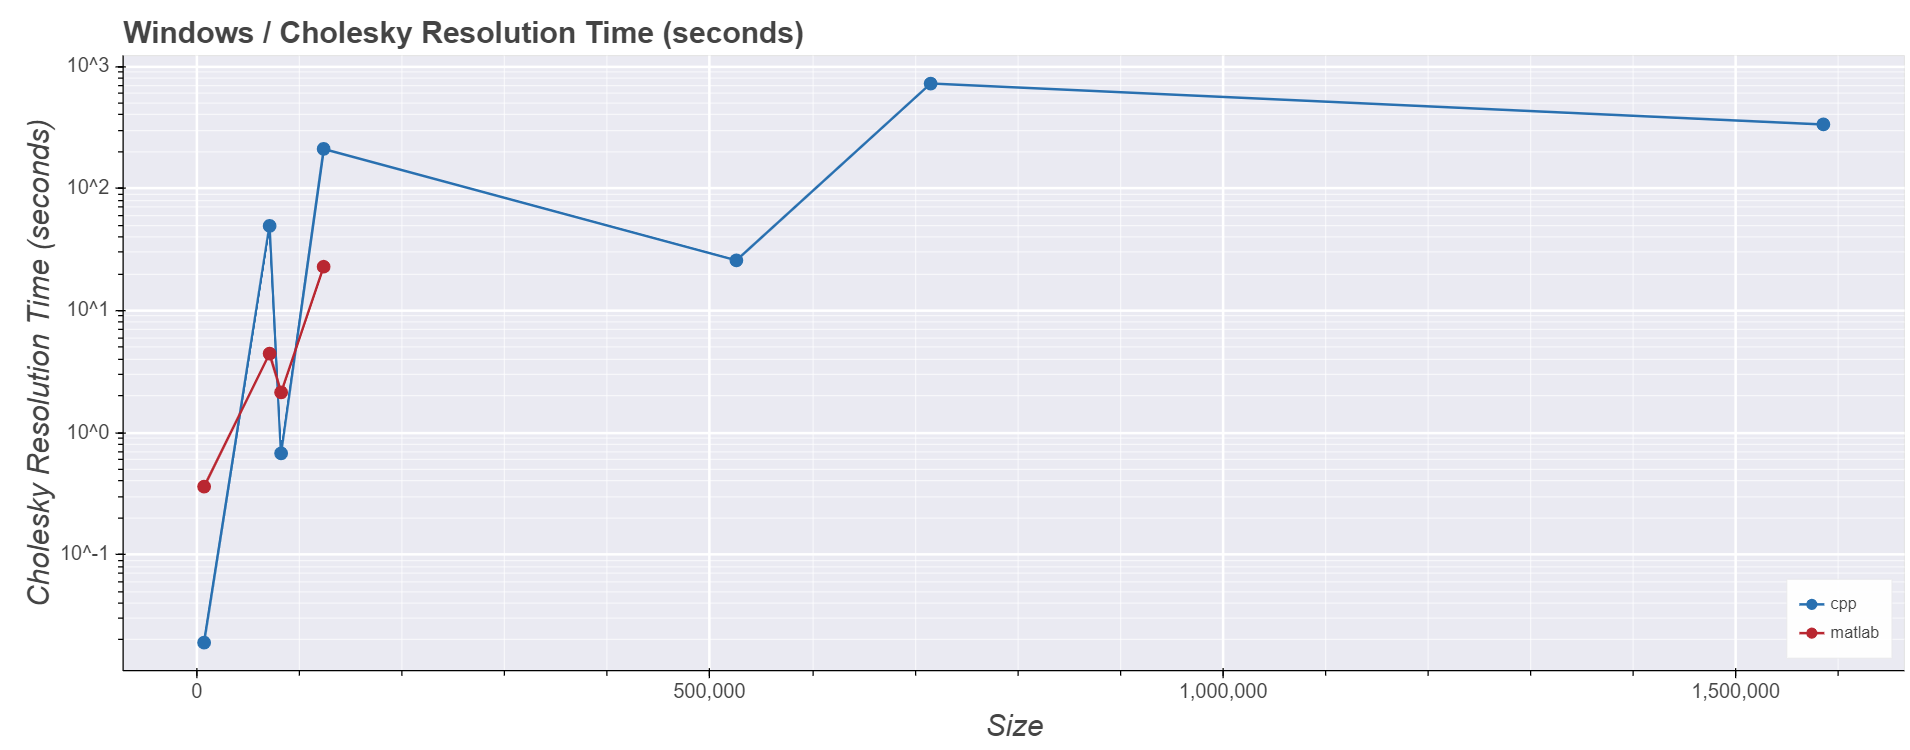
\includegraphics[width=1.3\linewidth]{windows_solve.png}}
    \caption{Tempo di risoluzione su Windows}
    \label{fig:windows-time}
\end{figure}

\smallskip
\subsubsection*{Memoria}
Come illustrato in \cref{fig:windows-memory}, l'implementazione in C++ occupa molta meno memoria rispetto a quella in MATLAB, in particolare al crescere della dimensione della matrice e del numero di elementi contenuti in essa.

Difatti, tutte le matrici analizzate in MATLAB per le quali non è presente un risultato nel grafico, durante la decomposizione di Cholesky hanno comportato un errore \lstinline{Out of memory}.
\begin{figure}[H]
    \makebox[\textwidth][c]{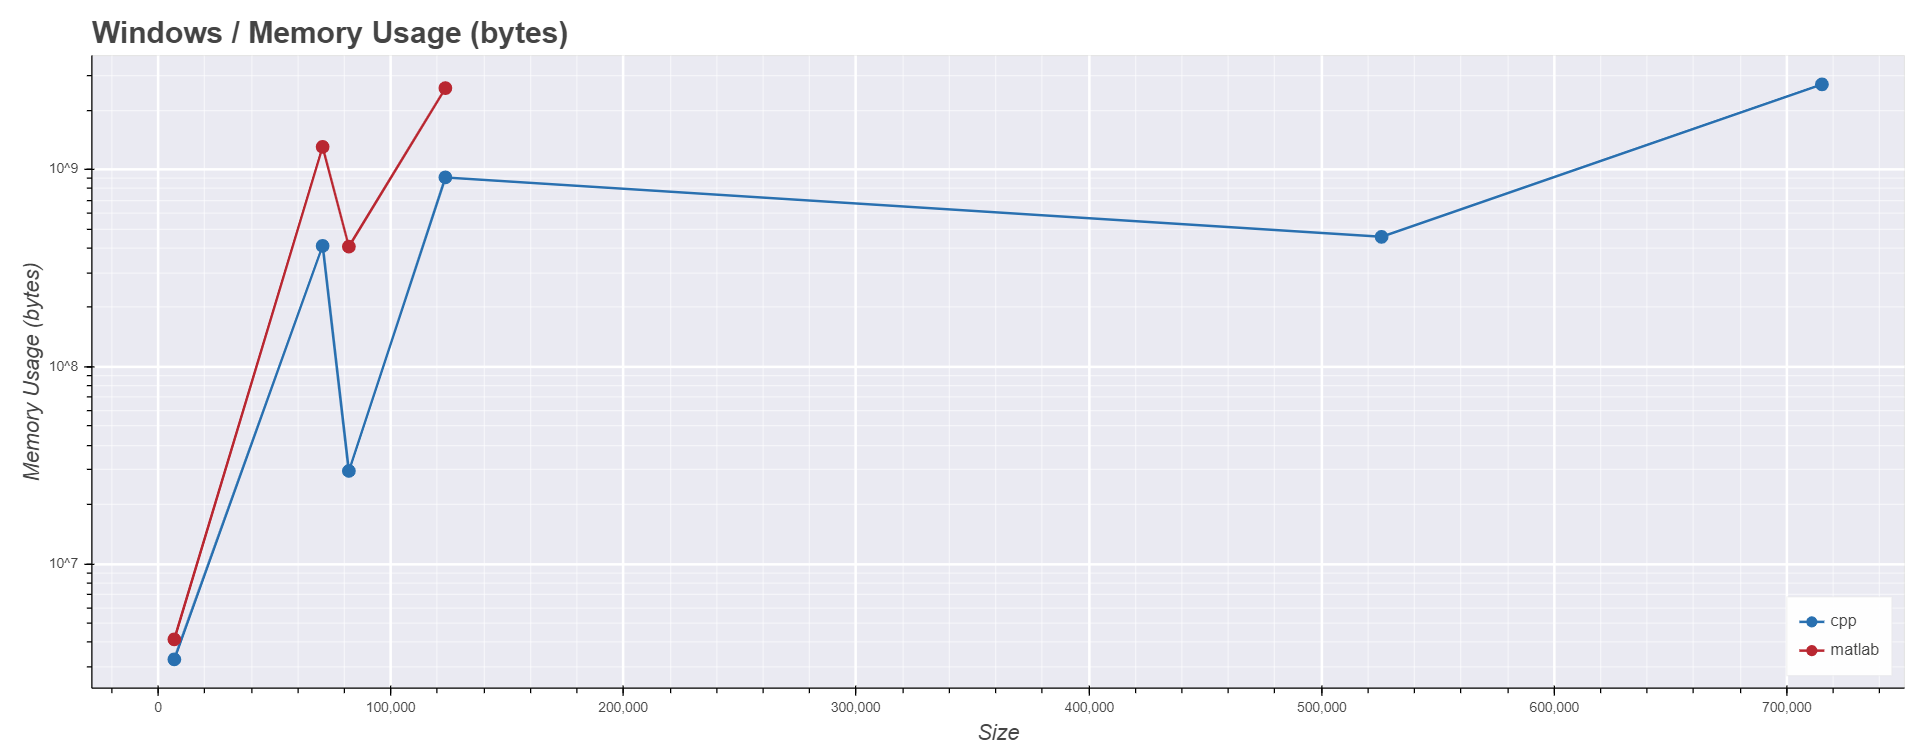
\includegraphics[width=1.3\linewidth]{windows_memory.png}}
    \caption{Utilizzo della memoria su Windows}
    \label{fig:windows-memory}
\end{figure}

\smallskip
\subsubsection*{Errore Relativo}
Entrambe le implementazioni presentano un errore relativo molto simile.
In \cref{fig:windows-error} si nota come al crescere della dimensione della matrice, in C++ l'errore relativo sembra stabilizzarsi tra $10^{-10}$ e $10^{-12}$.
\begin{figure}[H]
    \makebox[\textwidth][c]{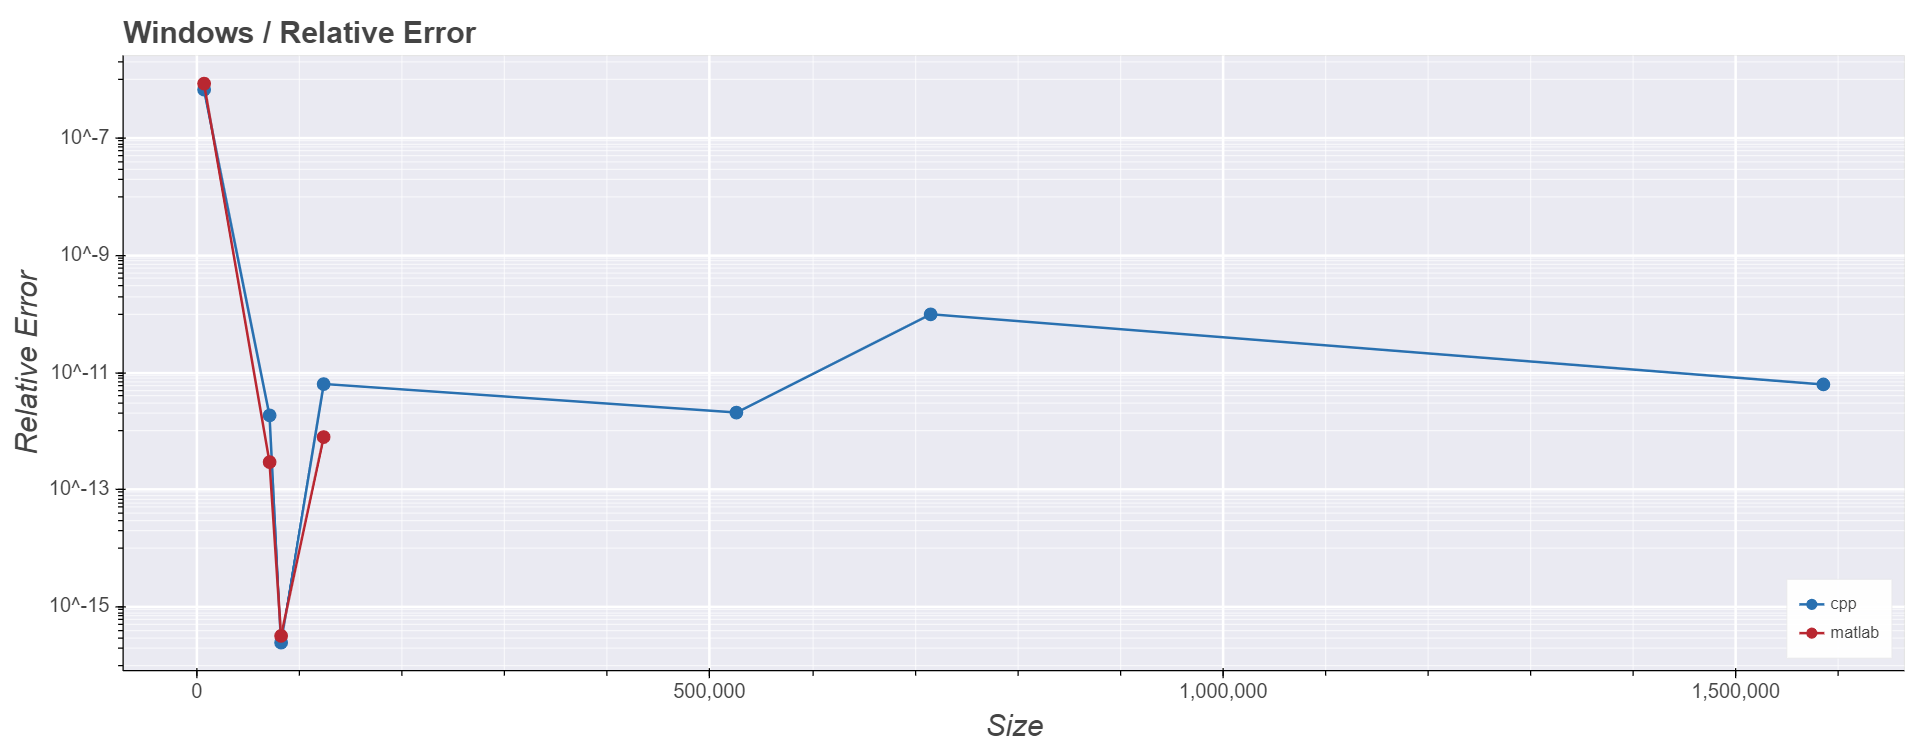
\includegraphics[width=1.3\linewidth]{windows_error.png}}
    \caption{Errore relativo su Windows}
    \label{fig:windows-error}
\end{figure}

\subsection{Linux}
\subsubsection*{Tempo}
L'andamento del tempo di risoluzione del sistema non risulta strettamente dipendente dalla dimensione della matrice. Inoltre, l'implementazione in MATLAB riesce a mantenere tempi di completamento meno variabili.
\begin{figure}[H]
    \makebox[\textwidth][c]{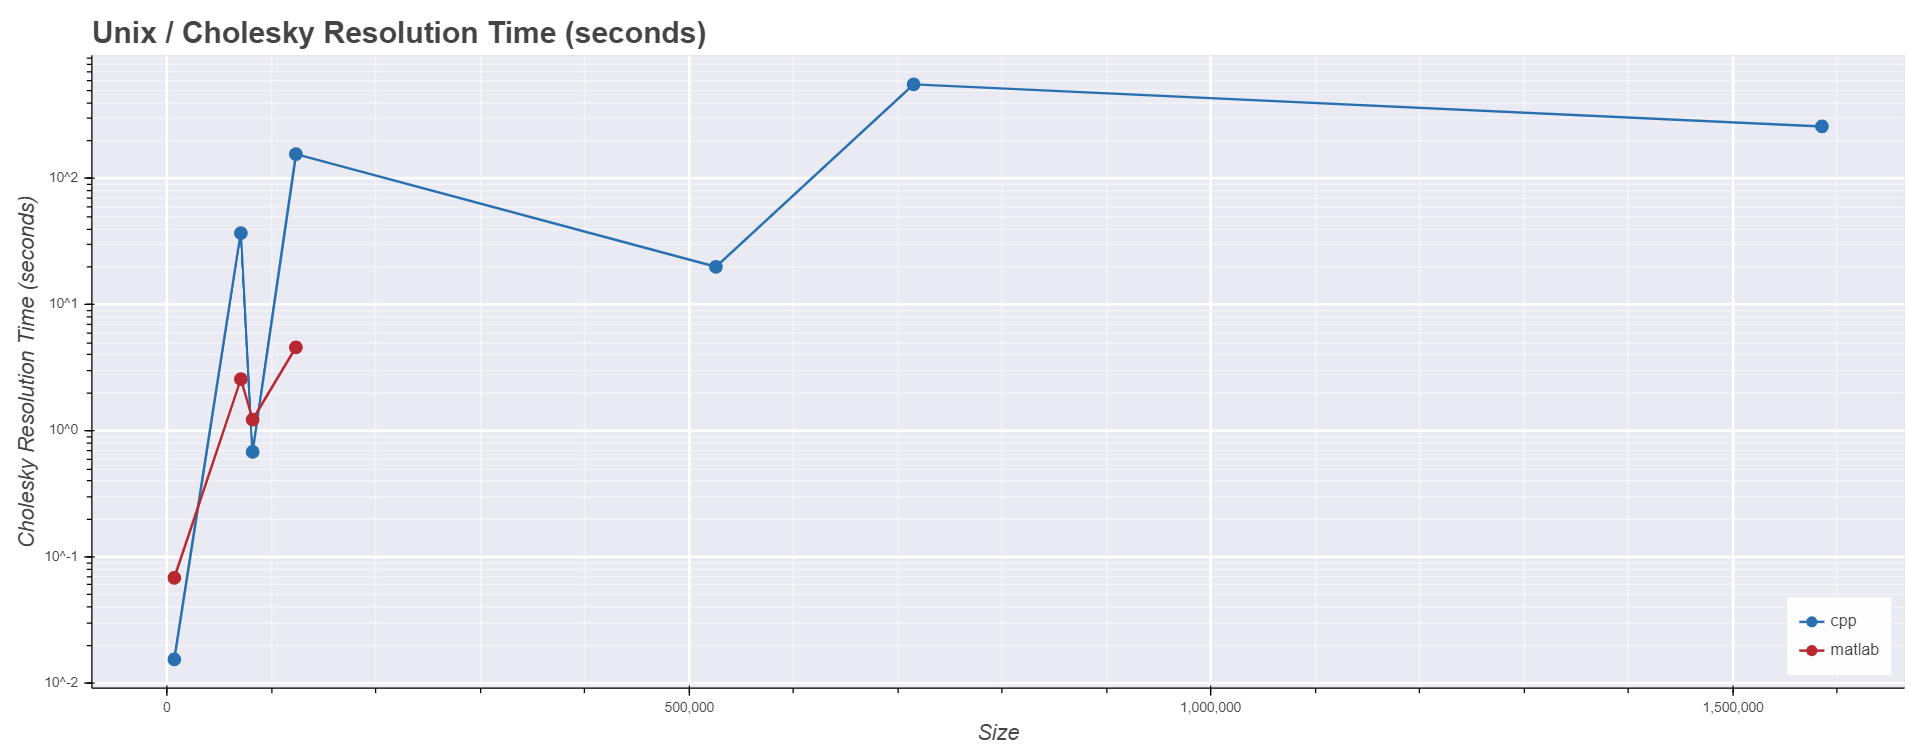
\includegraphics[width=1.2\linewidth]{unix_solve.png}}
    \caption{Tempo di risoluzione su Linux}
    \label{fig:linux-time}
\end{figure}

\subsubsection*{Memoria}
L'utilizzo della memoria, a differenza di quanto visto in precedenza nella \cref{fig:windows-memory} presenta una lettura iniziale molto bassa nell'implementazione MATLAB.
\begin{figure}[H]
    \makebox[\textwidth][c]{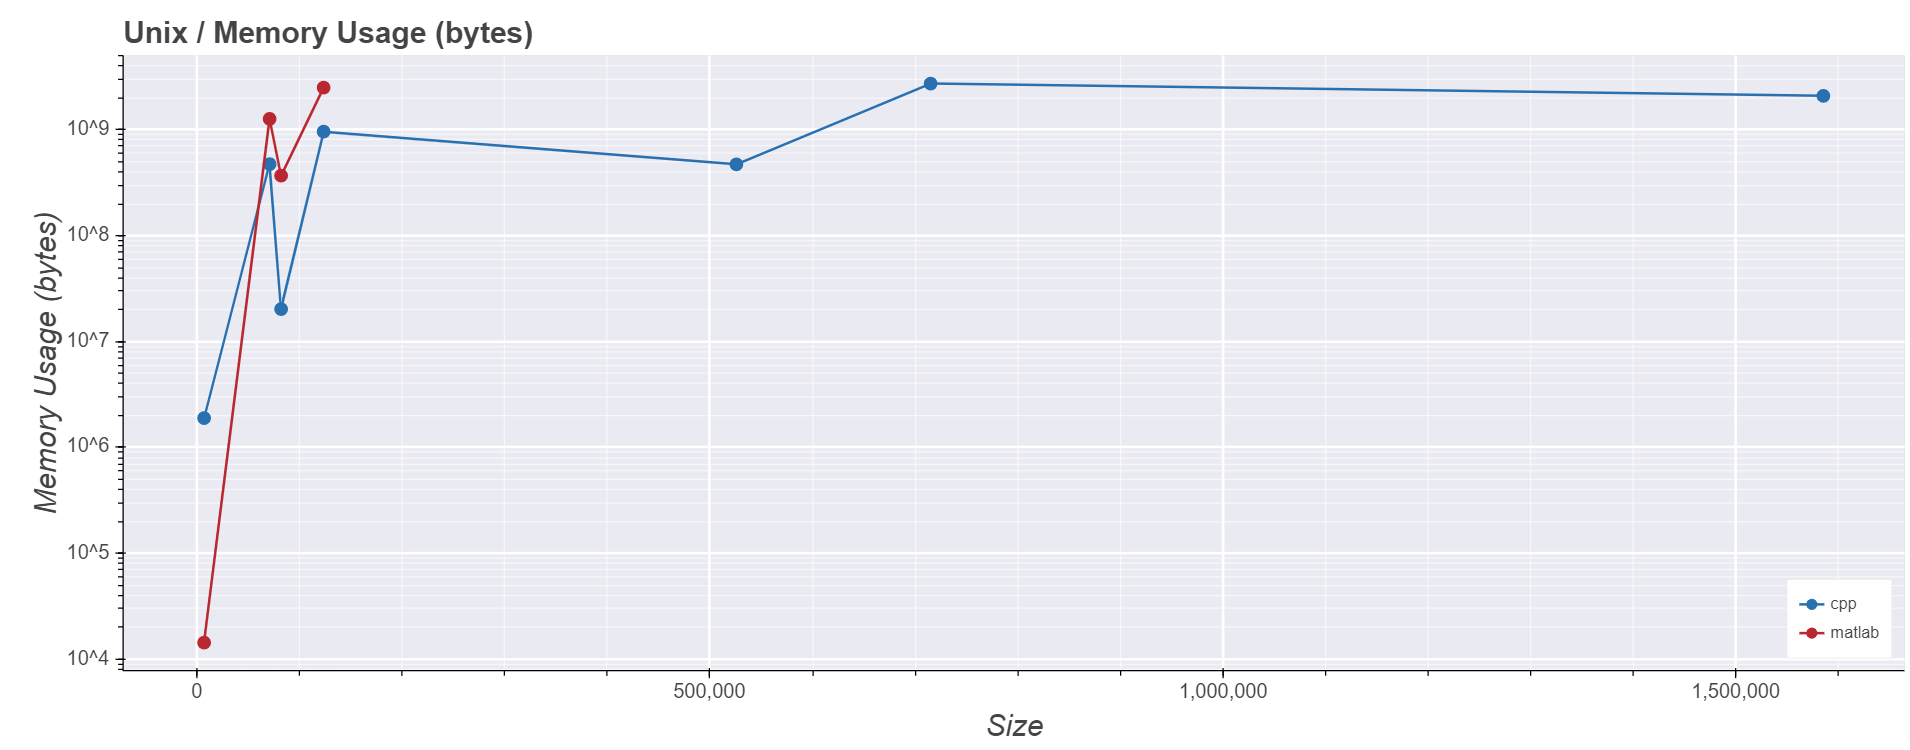
\includegraphics[width=1.2\linewidth]{unix_memory.png}}
    \caption{Utilizzo della memoria su Linux}
    \label{fig:linux-memory}
\end{figure}

\smallskip
\subsubsection*{Errore relativo}
Si nota che,sia su c++ che con la libreria MatLab, si ha un errore comparabile/quasi uguale per entrambi i metodi, e che dopo un massimo ed un minimo nelle matrici più piccole, l'errore si stabilizza intorno a $10^{-11}$, indipendentemente dalle dimensioni delle matrici che il programma riesce a caricare.
\begin{figure}[H]
    \makebox[\textwidth][c]{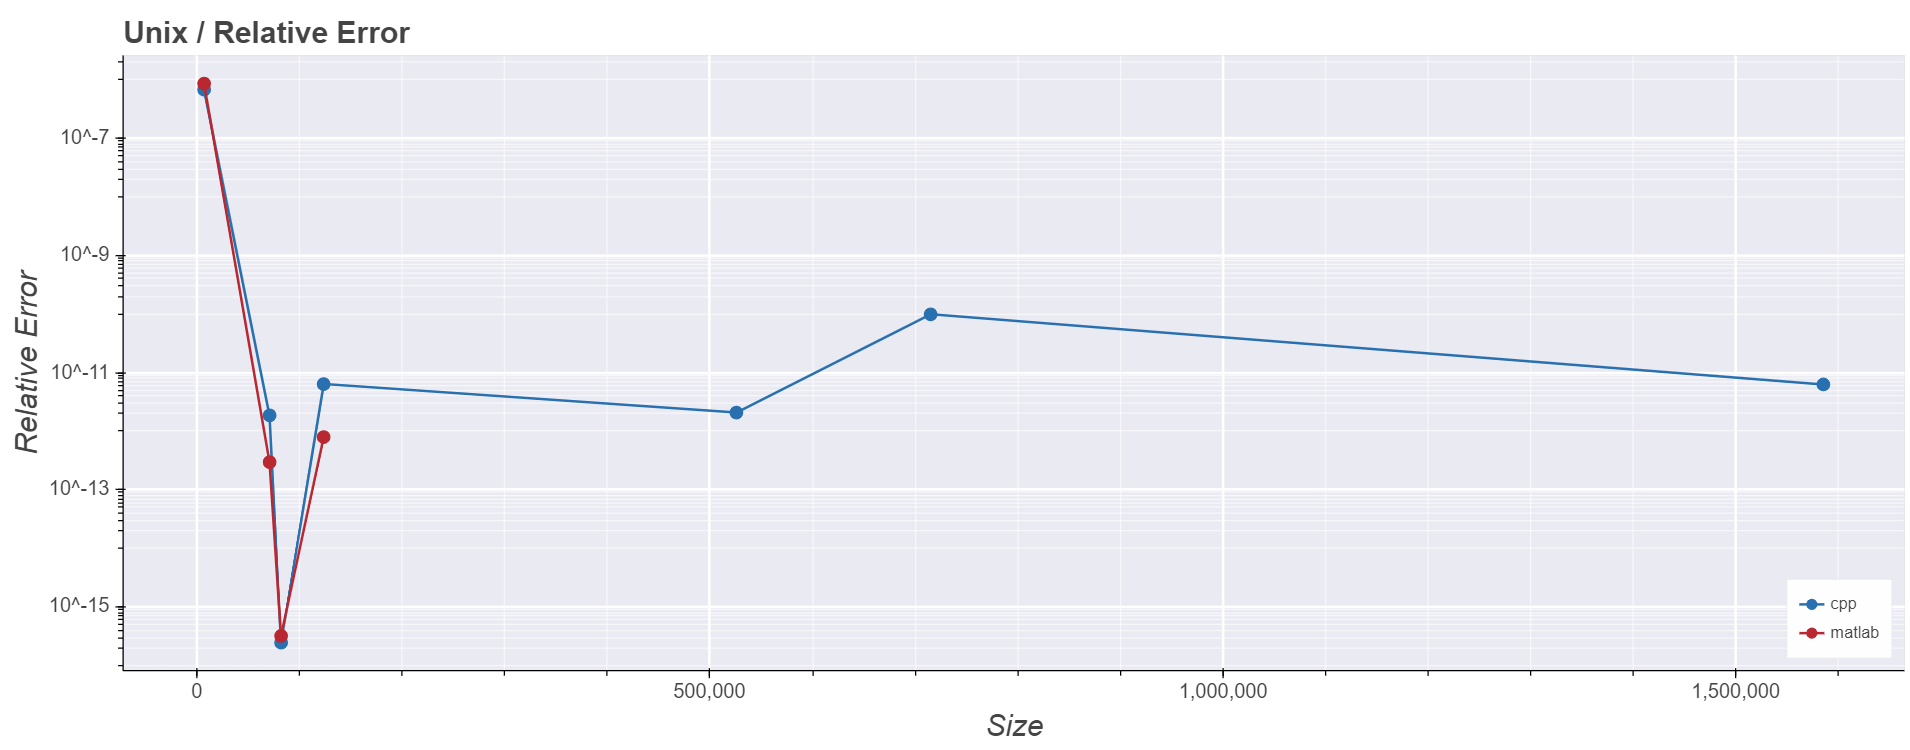
\includegraphics[width=1.3\linewidth]{unix_error.png}}
    \caption{Errore relativo su Linux}
    \label{fig:linux-error}
\end{figure}

\newpage
\section{Risultati per implementazione}
\label{section-results-os}

\subsection{C++}
\subsubsection*{Tempo}
TODO
\begin{figure}[H]
    \makebox[\textwidth][c]{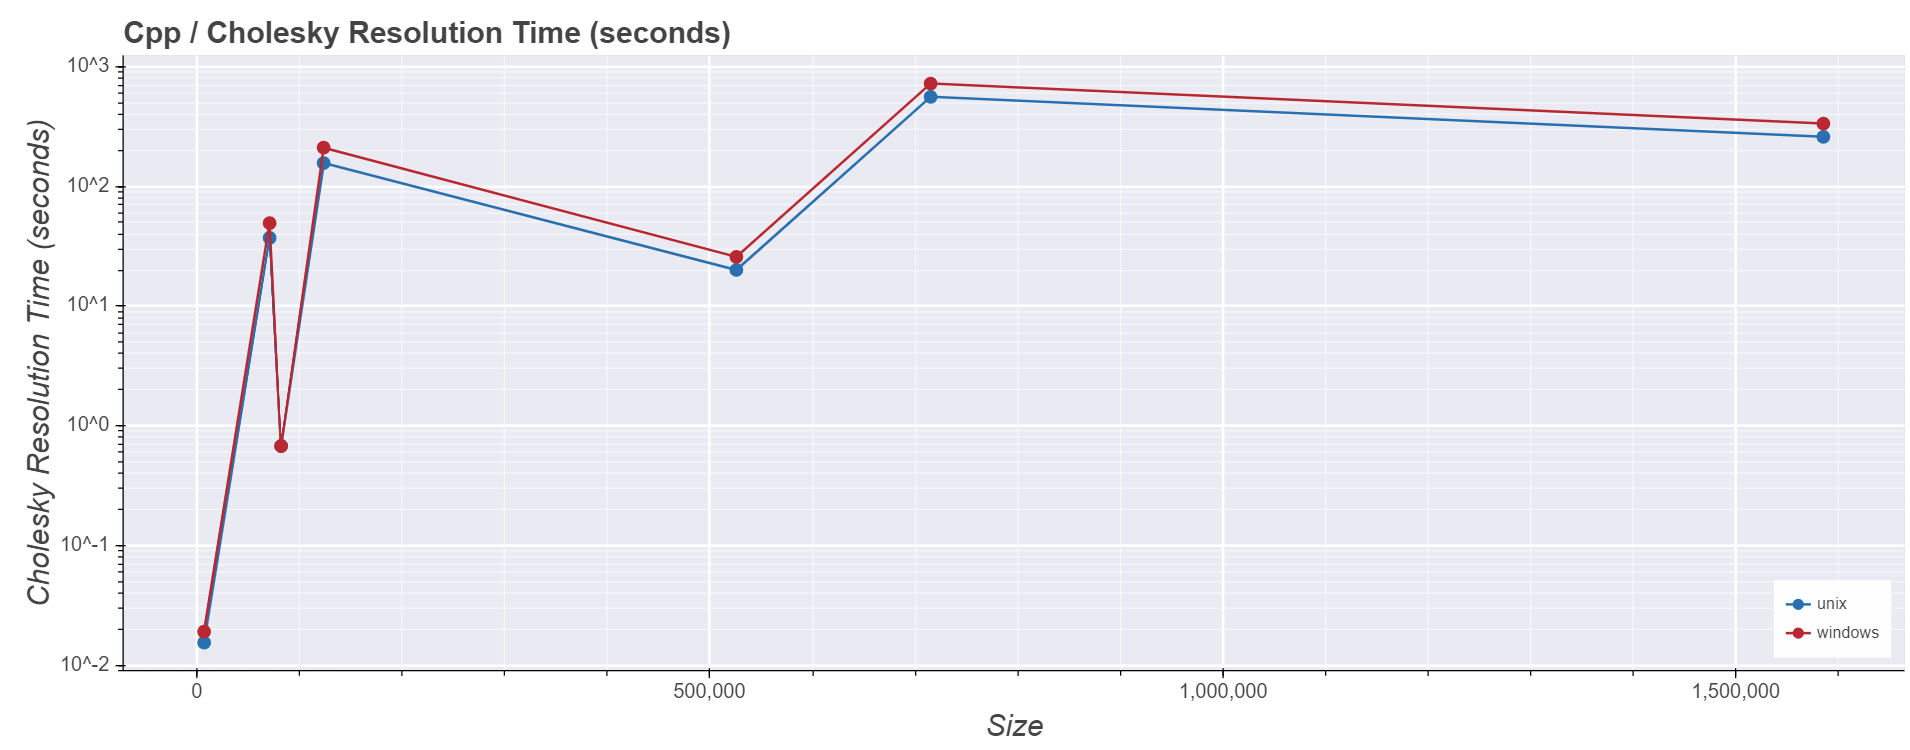
\includegraphics[width=1.3\linewidth]{cpp_solve.png}}
    \caption{Tempo di risoluzione nell'implementazione C++}
    \label{fig:cpp-time}
\end{figure}

\subsubsection*{Errore Relativo}
TODO
\begin{figure}[H]
    \makebox[\textwidth][c]{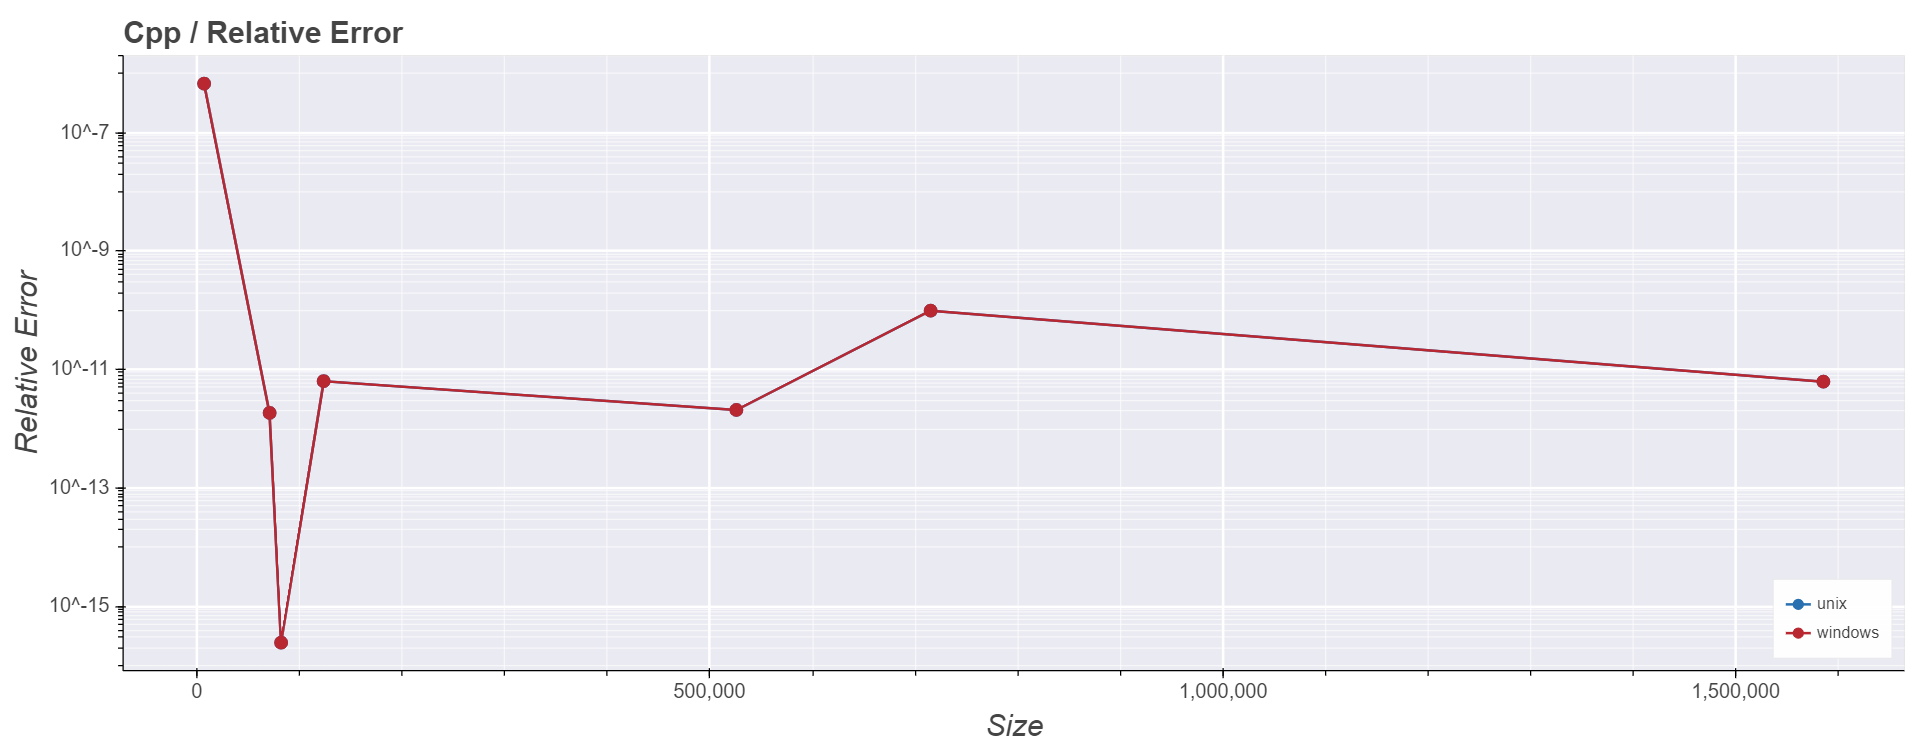
\includegraphics[width=1.3\linewidth]{cpp_error.png}}
    \caption{Errore relativo nell'implementazione C++}
    \label{fig:cpp-error}
\end{figure}

\subsubsection*{Memoria}
TODO
\begin{figure}[H]
    \makebox[\textwidth][c]{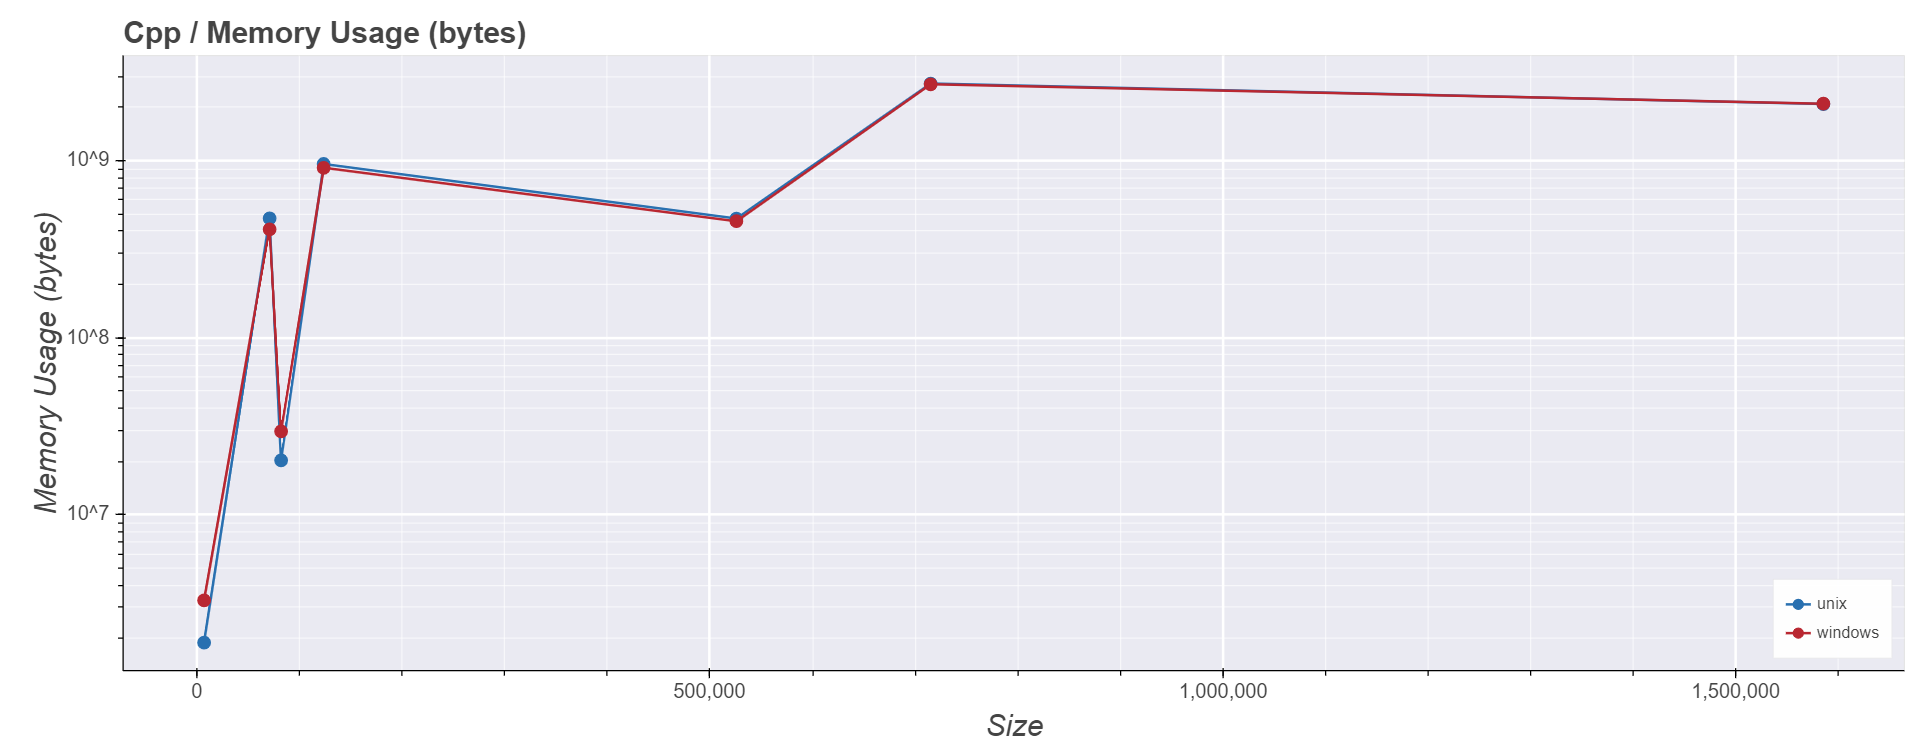
\includegraphics[width=1.3\linewidth]{cpp_memory.png}}
    \caption{Utilizzo della memoria nell'implementazione C++}
    \label{fig:cpp-memory}
\end{figure}

\subsection{Matlab}
\subsubsection*{Tempo}
TODO
\begin{figure}[H]
    \makebox[\textwidth][c]{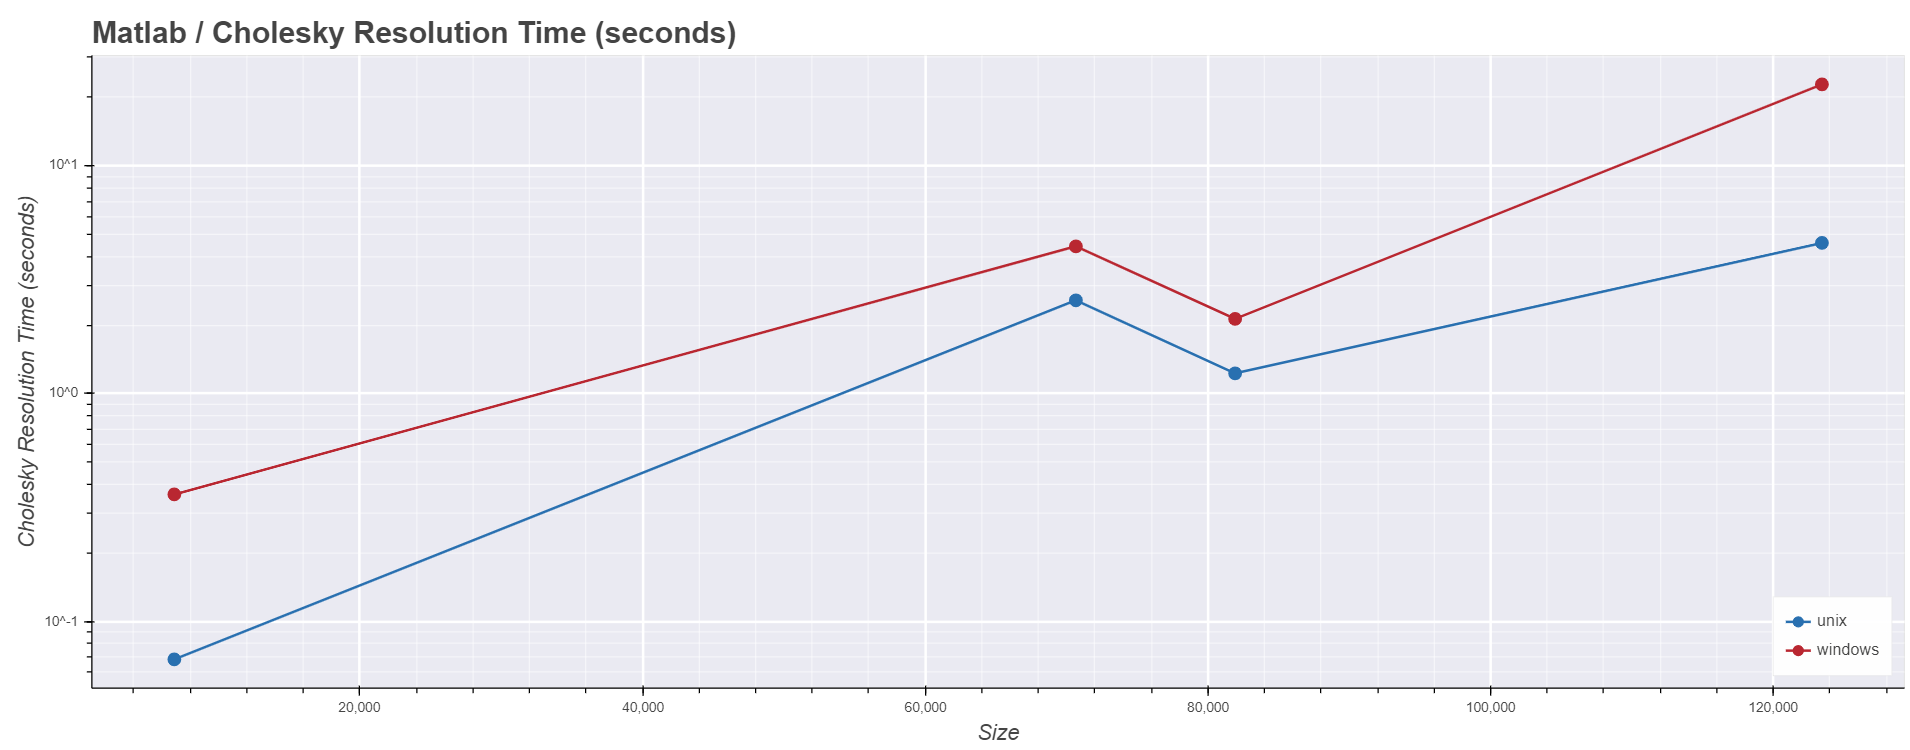
\includegraphics[width=1.3\linewidth]{matlab_solve.png}}
    \caption{Tempo di risoluzione nell'implementazione MATLAB}
    \label{fig:matlab-time}
\end{figure}

\subsubsection*{Errore Relativo}
TODO
\begin{figure}[H]
    \makebox[\textwidth][c]{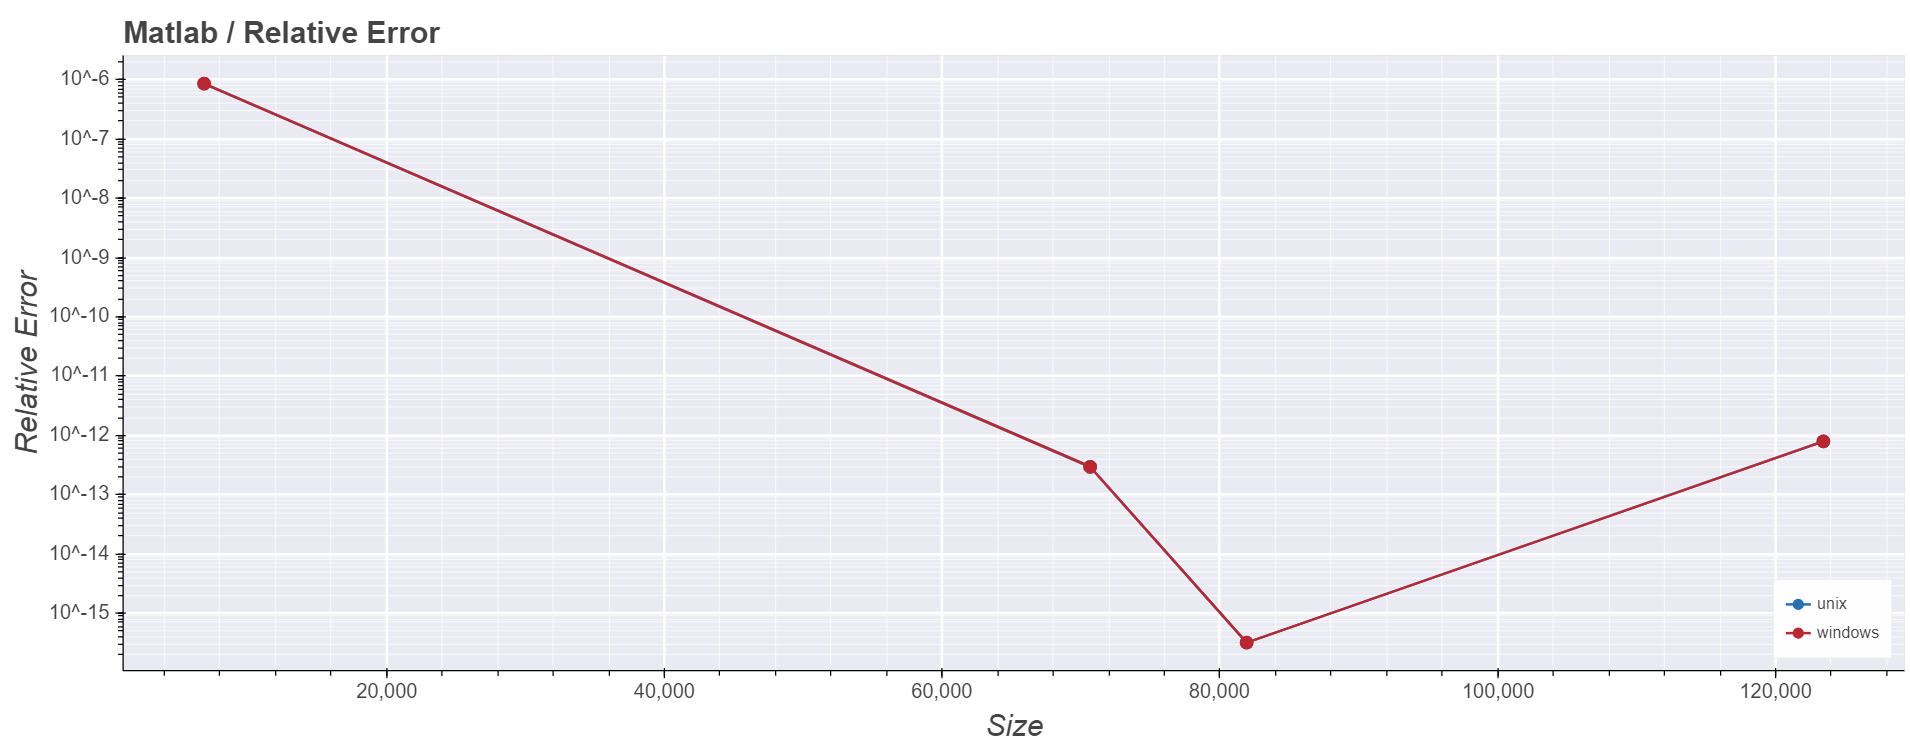
\includegraphics[width=1.3\linewidth]{matlab_error.png}}
    \caption{Errore relativo nell'implementazione MATLAB}
    \label{fig:matlab-error}
\end{figure}

\subsubsection*{Memoria}
TODO
\begin{figure}[H]
    \makebox[\textwidth][c]{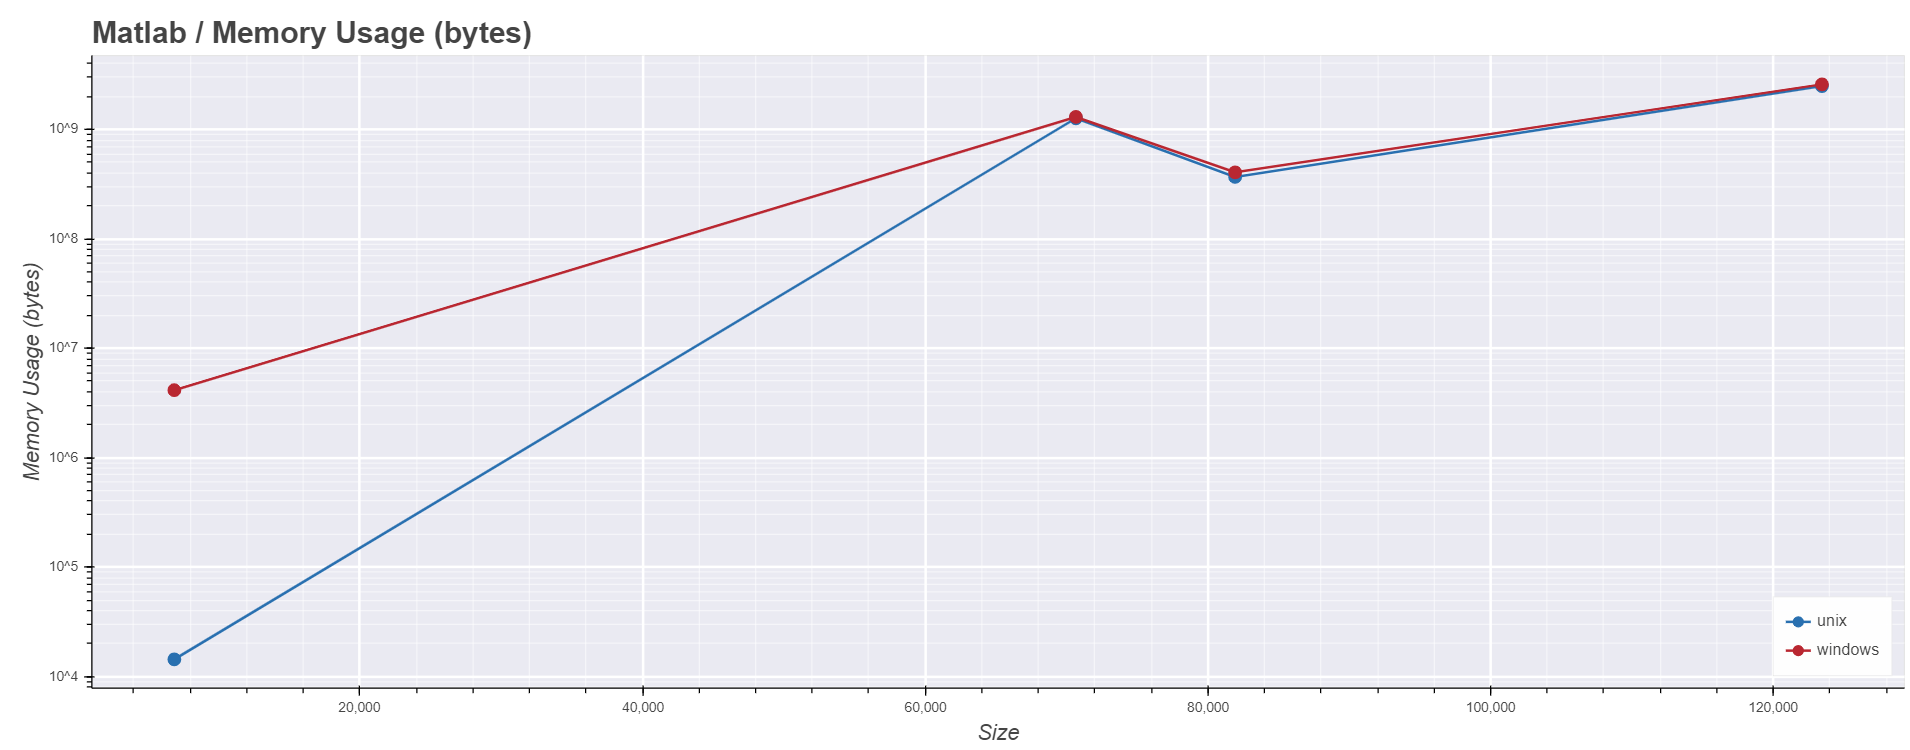
\includegraphics[width=1.3\linewidth]{matlab_memory.png}}
    \caption{Utilizzo della memoria nell'implementazione MATLAB}
    \label{fig:matlab-memory}
\end{figure}

\newpage
\section{Conclusioni}
TODO

\subsection{Suddivisione del lavoro}
Durante la realizzazione del progetto tutti i componenti del gruppo hanno partecipato attivamente alla sua realizzazione. In particolare:
\begin{itemize}
  \item \textbf{Edoardo Silva} si è occupato...
  \item \textbf{Davide Marchetti} si è occupato...
  \item \textbf{Bryan Zhigui} si è occupato...
\end{itemize}

\noindent
Tutti i componenti del gruppo hanno lavorato alla ... e collaborato alla stesura di questo documento.
\end{document}